\documentclass{stdlocal}
\begin{document}
\section{Design of the Library Interface} % (fold)
\label{sec:design_of_the_api}
  The design of a library API using various vectorized PRNGs consists of several parts, as can be seen in figure \ref{fig:api-parts}.
  To exploit the statistical properties of all the implemented generators proper seeding routines have to be provided.
  Seeding of PRNGs should be easy but not magically hiding important information, like the RNG that is used for the initialization.
  The implementation of the MT19937 given by \code{std::mt19937} in the STL of the C++ programming language for example, internally uses an easier PRNG to initialize its whole state vector by only one truly random number \autocite{gcc-libstdcpp}.
  The interface of \code{std::mt19937} does not show this information to the programmer or the reader and even forces the user of the library to employ this process.
  Furthermore, a generator \code{RNG} only used for seeding will typically be constructed directly as an rvalue in the constructor of the \code{std::mt19937}.
  \[
    \text{\code{std::mt19937 rng\{RNG\{\}()\};}}
  \]
  Because we cannot use the complete RNG as an argument, we first have to make sure that we call the advancing routine of the seeding generator.
  This behavior reduces the statistical performances of the initialization and complicates the interface even more by adding an extra pair of parentheses.

  \begin{figure}[b]
    \center
    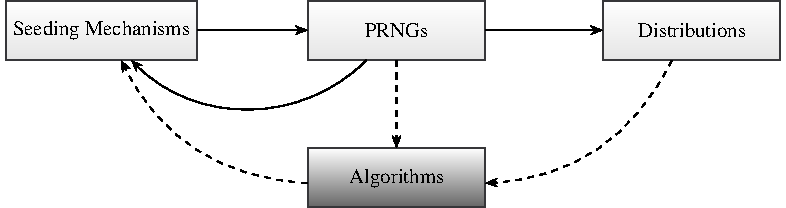
\includegraphics[width=0.95\textwidth]{figures/api_parts.pdf}
    \caption[Main Parts of the API Design]{
      Main parts to be considered for a software library that is providing access to scalar and vectorized PRNGs.
      The arrows show possible interactions between different parts for which convenient interfaces should be created.
      In this thesis, algorithms will not be considered.
    }
    \label{fig:api-parts}
  \end{figure}

  Other parts we have to deal with are fast and easy-to-use distributions for RNGs to at least generate uniform random numbers.
  The current C++ standard supplies different distributions in the form of functor templates that use the same algorithm for all generators by templatizing their function operators.
  \[
    \text{\code{std::uniform\_real\_distribution<float> dist\{\}; auto x = dist(rng);}}
  \]
  This API design consists of two major drawbacks.
  The user always has to first construct the object of the according distribution type and afterwards using its function operator to actually get a random number that fulfills the conditions of the distribution.
  Hence, even for simple use cases an API overhead emerges by utilizing random numbers via the STL of C++.
  The second problem is that every RNG has to use the same distribution routine which may not be optimized to work well with a given generator.
  Especially for uniformly distributed random numbers, some generators can exploit the implementation of their transition and generator function to achieve better performance.
  But in C++, we are not able to specialize the function operator template in a distribution functor from the outside.
  The approach does not scale well with the number of different RNGs.

  In the last few years, there has been some development in the area of API design for RNGs.
  \textcite{oneill-blog-api,oneill-blog-rd,cpp-std-seeding,cpp-std-random}, to name a few.
  They provide perfect basic ideas to improve the usage of random utilities in the C++ language.
  We will rely on this work and go a step further.
  We strive for a transparent API that can be used easily with different seeding alternatives.
  Nearly every RNG should be available as a source for seeding another RNG.
  In addition, uniform distribution functions will be introduced that do not need to be called as functor objects.
  Through template meta programming, we give generators the possibility of specializing such helper functions through member functions of the same name.
  This idea makes it even possible to specialize these functions outside of the RNG structure for a non-intrusive adjustment.
  Furthermore, by providing these functions we keep compatibility to the standard distributions.

  \subsection{Concepts} % (fold)
  \label{sub:prng_concept}
    We do not want to introduce a lot of overhead to the design concept of PRNGs and vectorized PRNGs.
    The compiler should automatically find out which algorithm to use.
    This can be done by specialization according to the result type of the function operator.
    If this should be not enough, tag dispatching can be used.

    The output could have arbitrary size but it is always interpreted as a finite length bit stream.
    For AVX this means a $256\appendUnit{bit}$ stream.
    This explains how to interleave SIMD streams and how to test them.

    Interfaces for SIMD intrinsics will always be specialized templates even for wrapper classes because SIMD is behaving differently to SISD architectures.
    If we are working with SIMD vector the least surprising interface is to use the SIMD vector as result type directly.
    Through inheritance we or someone from the outside could add another interface by using wrapper classes without changing the implementation.
    Therefore seeding will be a specialized routine.
  % subsection prng_concept (end)

  \subsection{Template Utilities} % (fold)
  \label{sub:utilities}
    The ideas for the API given above require us to rely on the template meta programming facilities C++ provides.
    In general, we would like to use helper functions, as well as member functions for specific tasks, like generating a vector of random numbers.
    If a generator provides a member function the helper function should use the given specialization whereas otherwise a default algorithm should be used.
    Hence, at compile-time we need to evaluate if calling a specific member is a valid expression.
    In \textcite{vandevoorde2018}, there is a given technique that allows us to evaluate the validity of expressions.

    \inputCodeBlock[title = Is-Valid Utility]{code/is_valid.hpp}
    This code highly makes use of template meta programming artifacts, like SFINAE and type traits.
    To be precise, it uses an overloaded variadic helper function template \code{detail::is\_valid} to decide if the call of a specific function type \code{F} with the varying amount of argument types \code{Args} would be a valid call.
    The call is put into an unevaluated context by using the \code{std::declval} template utility from C++ which is able to return an object of a class without specific constructors in such an unevaluated context.
    To decide the validity of this statement it relies on a default template parameter and the \code{decltype} utility of the C++ language.
    If the call to the given function object would be possible, \code{decltype} will indeed deduce the return type of the function call and correctly set the default template argument.
    In this case, the first overload would be chosen so that the return type of \code{detail::is\_valid} would be \code{std::true\_type}.
    In all other cases, the second overload with the return type \code{std::false\_type} would be activated because due to SFINAE the first overload would not be taken into account.
    We have to make sure to decide on the validity with the generalized boolean types \code{std::true\_type} and \code{std::false\_type} from the STL of C++ because we will use the given templates in unevaluated contexts where no evaluation of an actual \code{bool} variable would be possible.

    The routine \code{is\_valid} is actually a lambda expression that returns another lambda expression which is then evaluating the validity of its arguments by the helper template \code{detail::is\_valid}.
    The function object \code{f} will be a lambda expression that lists conditions for abstract types which have to be valid to fulfill the concept we want to define.
    The arguments \code{args} will then be the actual variables to be inserted in the pattern test of \code{f}.
    The two interleaved lambda expressions separate the function object \code{f} from its varying amount of arguments \code{args} for convenience.
    Additionally, they allow us to use variables in unevaluated contexts.

    To better understand the utility, we will directly apply it to construct a helper function template \code{generate} which is calling \code{std::generate} from the STL of C++ for a given RNG as a default.
    But as a specialization we would like to call the member function with the same name of the generator if it exists.
    We do this again through the use of SFINAE.

    \inputCodeBlock[title = Generate Utility]{code/generate.hpp}
    First, we are defining a general pattern \code{has\_generate} based on \code{is\_valid} to be able to decide the validity of the expression \code{x.generate(y,z)} for arbitrary types by using a lambda expression.
    Again, we have to make sure the lambda expression is deducing its return in an unevaluated context.
    Hence, \code{decltype} is used as a trailing return type with the pattern to evaluate.
    Next, we declare an overloaded helper function template \code{generate}.
    SFINAE is applied for overload resolution by using \code{std::enable\_if\_t} in the return type of the functions.
    In the template argument, we use the general pattern \code{has\_generate(rng,first,last)} and deduce its type by \code{decltype}.
    The type will either be \code{std::true\_type} or \code{std::false\_type}.
    In the first case, \code{std::enable\_if\_t} will be evaluated to be the type \code{void}.
    In the other case, \code{std::enable\_if\_t} will be no valid type and the function will not be taken into account in the overload resolution.
    The overloads of \code{generate} use complementary conditions in the template argument of \code{std::enable\_if\_t}, so that at all times only one of them will be available in the overload resolution.
    As a result, \code{generate(rng,first,last)} will call \code{rng.generate(first,last)} if the type of \code{rng} provides the named member function and \code{std::generate(first,last,std::ref(rng))} otherwise.
  % subsection utilities (end)

  \subsection{Seeding Mechanism} % (fold)
  \label{sub:seeding}
    Seeding of RNGs through the use of other RNGs will be accomplished by the use of perfect forwarding.
    In contrast to the ideas in \textcite{cpp-std-seeding}, we allow for rvalue initialization making the API simpler.
    Consider the following code snippet that introduces an arbitrary RNG type \code{rng\_type}.

    \inputCodeBlock[title = Seeding Strategy]{code/seeding.hpp}
    \code{rng\_type} is a structure with an explicit forwarding constructor available for seeding which is able to match any other RNG type.
    Please note the typical usage of a universal reference to deduce forwarding types.
    The implementation of the constructor should call either the \code{generate} method or the function operator of the given RNG type to initialize its own state.
    For a few exceptional cases, the given code can lead to certain artifacts in the template deduction process.
    This behavior is discussed in \textcite[\ppno~188-197]{meyers2014}.
    For RNGs, there is typically no need to provide an extra degree of type security.
    But we can easily add it through the use of \code{std::enable\_if\_t} to turn on the SFINAE process.

    \inputCodeBlock[title = Advanced Seeding Strategy]{code/seeding_advanced.hpp}
    This implementation removes the explicit forwarding constructor for seeding when we want to copy or move the state of the structure itself.
    For the implementations of PRNGs, we have tested both variants and could not spot any differences.
    Hence, further we will use the simpler variant.
    According to \textcite{vandevoorde2018}, in the future of C++ concepts will be available which will make such an initialization artifact even simpler and more efficient.
  % subsection seeding (end)

  \subsection{Uniform Distribution Functions} % (fold)
  \label{sub:distributions}
    The design of a uniform distribution \code{uniform} via helper functions and member specializations will be handled the same way as for the function template \code{generate}.
    This time, we only have to take care of additional overloads.
    By calling \code{uniform} without function arguments, we have to provide the return type as a template argument.
    For floating-point types, the result should be a number in the interval $[0,1)$.
    Specifying integer number types, the output is a value of the complete range of the template argument.
    If we call \code{uniform} with additional arguments specifying the range of the output, we are able to use template argument deduction for the return type based on the range arguments.
    We separate those two cases to further optimize the frequently used first function call without arguments.
    % The following code shows the implementation.

    \inputCodeBlock[title = Uniform Template Is-Valid Patterns]{code/uniform_patterns.hpp}
    We use two \code{is\_valid} patterns to describe the existence of \code{uniform} member functions with and without additional arguments.
    The actual \code{uniform} functions then use the same overload resolution via SFINAE as the \code{generate} function.

    \inputCodeBlock[title = Uniform Template]{code/uniform.hpp}
    The result type of the Mersenne Twister \code{std::mt19937} from the STL is given by \code{uint\_fast32\_t} which, on modern machines, will evaluate to \code{uint64\_t} with $64\appendUnit{bit}$ size instead of the used $32\appendUnit{bit}$.
    Because the uniform distribution utilities that we will provide in the implementation use their argument types to overload themselves, the Mersenne Twister would call the wrong function.
    We can prohibit this behavior without changing the inner structure of the \code{std::mt19937} type by creating another helper function overload especially for the Mersenne Twister.
    In this implementation, we are making sure its return type will be casted to the \code{uint32\_t} type.

    \inputCodeBlock[title = Uniform MT19937 Overload]{code/uniform_mt19937.hpp}
    The defined API gives us the ability of a powerful default distribution together with the possibility of specializing it for some generators through member functions.
    If we cannot access the inner structure of an RNG then we may even insert slightly more complicated helper specializations to adjust the output of RNGs which are not created by the programmer itself.
  % subsection distributions (end)

  % \subsection{Algorithms} % (fold)
  % \label{sub:algorithms}

  % subsection algorithms (end)
\end{document}